%!TEX root = main.tex

%\subsection{From {\AMASS} models to FSMs of \nuxmv}\label{sec:amass2fsm}
%In Section~\ref{sec:apk2amass}, we show how to extract {\AMASS} models from APK files. 
In this section, we show how to encode the semantics of these {\AMASS} models into the reachability problem of finite state machines  that can be %discharged 
tackled by the symbolic model checker nuXmv \cite{CavadaCDGMMMRT14}. 
%
This encoding will facilitate the automated validation of the formal semantics of {\AMASS} models (Section~\ref{sec:validation}) and static analysis of Android apps (Section~\ref{sec:static}).

%In this section, we shall show how to incorporate the semantics of these {\AMASS} models into GUI testing and static analysis of Android apps, so that the testing coverage and analysis precision can be improved.

In general, {\AMASS} models are infinite-state systems, since %the heights of 
both the number of tasks (stacks) and the heights of stacks can be unbounded. We impose two predefined upper bounds, i.e., $c_t$ on the maximum number of tasks of the same affinity, and $\hbar$ on the height of stacks. As a result, we can obtain %turn {\AMASS} models into 
a finite state system. 
%, which can then be incorporated into the automated validation of formal semantics of {\AMASS} models and static analysis of Android apps. 
%
Nevertheless, even with these upper bounds, %the number of tasks and the heights of stacks are bounded, 
the number of configurations of an {\AMASS} model can be \emph{exponential} in the size of the model and $c_t$ and $\hbar$, %which hinders efficient validation of formal semantics and  static analysis. 
%To tackle this %the exponential state space blowup 
for which we resort to % the well-known symbolic model checker 
nuXmv \cite{CavadaCDGMMMRT14} and translate an {\AMASS} $\Mm$ (with given $c_t$ and $\hbar$) to an FSM $\Aa_\Mm$. 
%As a result, we encode the finite state systems corresponding to the {\AMASS} model  into a finite state machines (FSM) to feed to nuXmv. 

%The configuration reachability problem is formally defined as follows: Given an ASM $\Aa$ and a configuration $\rho$, decide whether $ ([A_0], 1) \xRightarrow{\Aa} (\rho, \ell)$ for some $\ell$, where $\xRightarrow{\Aa}$ is the reflexive and transitive closure of $\xrightarrow{\Aa}$. Note here we ignore the components $(\tau, i)$ in tuples $(\rho, \ell) \xrightarrow[\tau, i]{\Aa} (\rho', \ell')$ and take $\xrightarrow{\Aa}$ as a binary relation over $\conf_\Aa \times \natnum$.
%
%
%Our general approach is to translate an {\AMASS} $\Mm$ with a constant bound $c_t$ over the number of tasks of the same affinity and 
%a constant bound $\hbar$ over heights of stacks to an FSM $\Aa_\Mm$.

In \nuxmv, an FSM  $\Aa$ is triplet
$(\vec{x}, \vec{s}, \delta)$, where 
\begin{itemize}
\item $\vec{x}$ is a tuple of Boolean variables representing the inputs, 
\item $\vec{s}$ is a tuple of Boolean variables representing the states,  
\item $\delta$ is a Boolean formula involving the variables $\vec{s}$, $\vec{x}$, and $\vec{s'}$ to describe the transitions, where $\vec{s'}$ is a tuple of primed state variables that represent their new values after a transition.
 %involving the variables 
%$V(s)$ is a value set of the variable $s$ (resp. $x$) in $\vec{s}$ (resp. $\vec{x}$),  (resp. $Vx$).
%\item $\phi_i$ is a boolean formula involving the variables $\vec{s}$ to specify the set of initial states,
%\item $\phi_f$ is a boolean formula involving the variables $\vec{s}$ to specify the set of final states.
\end{itemize}
%$I(\vec{s})$ (resp. $O(\vec{s})$) is a boolean formula involving the variables $\vec{s}$ to specify the set of initial states (resp. final states), 
%
%$\delta(\vec{s}, \vec{x}, \vec{s'})$, called the transition relation, is a boolean formula over %involving the variables 
%$\vec{s}$, $\vec{x}$, and $\vec{s'}$ to describe how inputs lead from one state to possibly many different states. (Here $\vec{s'}$ is the tuple of primed variables corresponding to $\vec{s}$.)  

%For instance, let $\Mm_{\nuxmv} = (\vec{x}, \vec{s}, I, O, T)$ be the FSM, 
%where $\vec{s} = (s_1)$, $\vec{x} = (x_1)$, $V(s_1):= \{a_1,a_2\}$, $V(x) = \{0,1\}$, $I(\vec{s}) :=  (s_1=a_1)$, $O(\vec{s}):= (s_1=a_2)$, $T(\vec{s}, \vec{x}, \vec{s'}) = ((s_1=a_1) \wedge (x_1=1) \wedge (s'_1=a_2)) \vee ((s_1=a2) \wedge (x_1=0) \wedge (s'_1=a1))$, then $\Mm_{\nuxmv}$ accepts the language $(10)^*1$.

Let $\Mm = (\act, A_0,\frag, \vgr, \lmd, \aft,  \Delta)$ be an {\AMASS} and $\conf_{\Mm, c_t, \hbar}$ denote the set of configurations of $\Mm$ where 
the number of tasks of the same affinity is no more than $c_t$ and 
the heights of all stacks are no more than $\hbar$. It follows that $(\conf_{\Mm, c_t, \hbar}, \xrightarrow{\Mm})$ is a finite state system.\footnote{Strictly speaking, $\xrightarrow{\Mm}$ should be the restriction of $\xrightarrow{\Mm}$  to $\conf_{\Mm, c_t, \hbar}$}
Then we show how to encode $(\conf_{\Mm, c_t, \hbar}, \xrightarrow{\Mm})$ into an FSM $\Aa_\Mm$.
%
Intuitively, the states of $\Aa_\Mm$ represent the configurations in $\conf_{\Mm,c_t, \hbar}$ and the transitions of $\Aa_\Mm$ %mimics 
simulate the transition rules of $\Mm$. %to update the configurations of $\Aa$.
%

To facilitate the encoding, we first introduce the following definitions. % some numbers related to $\Mm$.
\begin{itemize}
\item Let $k_c$ denote the maximum length of $\vgr(A)$ for $A \in \act$, that is, the maximum number of fragment containers in an activity. 
%
\item Let $k_a$ denote the maximum number of actions occurring in the fragment transaction of one transition rule of $\Mm$.
%
\item Let $X$ denote the set of variables occurring in the transitions of $\Mm$ for storing the identifiers of fragment instances and $k_i = |X|$.
%
\item Let $k_t = c_t|\aft(\act)|$, namely, the maximum number of tasks in the task stacks. 
\end{itemize}


Recall that each configuration in $\conf_{\Mm}$ is 
$\rho=((S_1,A_1,b_1), \cdots, (S_n,A_n,b_n))$.
Let 
%
$$\Sigma_{\Mm} = \act \cup \frag \cup \{\ADD, \REM\} \cup  \cid_\Mm \cup X \cup [k_c\hbar]  \cup \{0,1, \bot\},$$ 
%
where $\cid_\Mm$ is the set of fragment container identifiers occurring in $\Mm$ and $\bot$ is a dummy symbol introduced as placeholders. 
Then each task stack in $\conf_{\Mm, \hbar}$ can be encoded by a word of length \emph{exactly} 
%
$k_t(2+\hbar (1+k_c \hbar + 4k_a \hbar(\hbar+1)+k_i))$
%
over the alphabet $\Sigma_{\Mm}$.
The arguments for this fact go as follows (see Figure~\ref{fig-conf-enc} for an illustration): 
\begin{itemize}
\item According to the semantics of {\AMASS}, $\rho$ contains at most $k_t$ tasks, that is, $n \le k_t$.  
%
\item Suppose $S_i = [(B_{i,1}, \Theta_{i,1}), \cdots, (B_{i, l_i}, \Theta_{i, l_i})]$, and for each $i \in [n]$ and $j \in [l_i]$, $\Theta_{i, j} = (\upsilon_{i,j}, \eta_{i,j}, \iota_{i,j})$. Then for each $i \in [n]$, $l_i \le \hbar$, moreover, for each $j \in [l_i]$, $\upsilon_{i,j}$ contains at most $k_c$ fragment containers and the height of each of them is no more than $\hbar$, and $\iota_{i,j}$ is a function from $X$ to $\{0\} \cup [k_c\hbar]$ (since each fragment contains at most $\hbar$ instances in one fragment container and there are at most $k_c$ fragment containers). 
%
\item Furthermore, $\eta_{i,j}$ contains at most $\hbar$ transactions, each of which has at most $k_a(\hbar+1)$ concretized actions. To see this, note that $\eta_{i,j}$ is obtained by concretizing at most $k_a$ actions in some transition rule of $\Mm$ and each such action is concretized into at most $\hbar + 1$ actions (because the heights of the history contents of fragment stacks are no more than $\hbar$). Note that each action $\beta(F', i', n')$ in the transactions of $\eta_{i,j}$ is encoded by a word of length $4$.
\end{itemize}
%
\begin{figure*}[t]
\centering
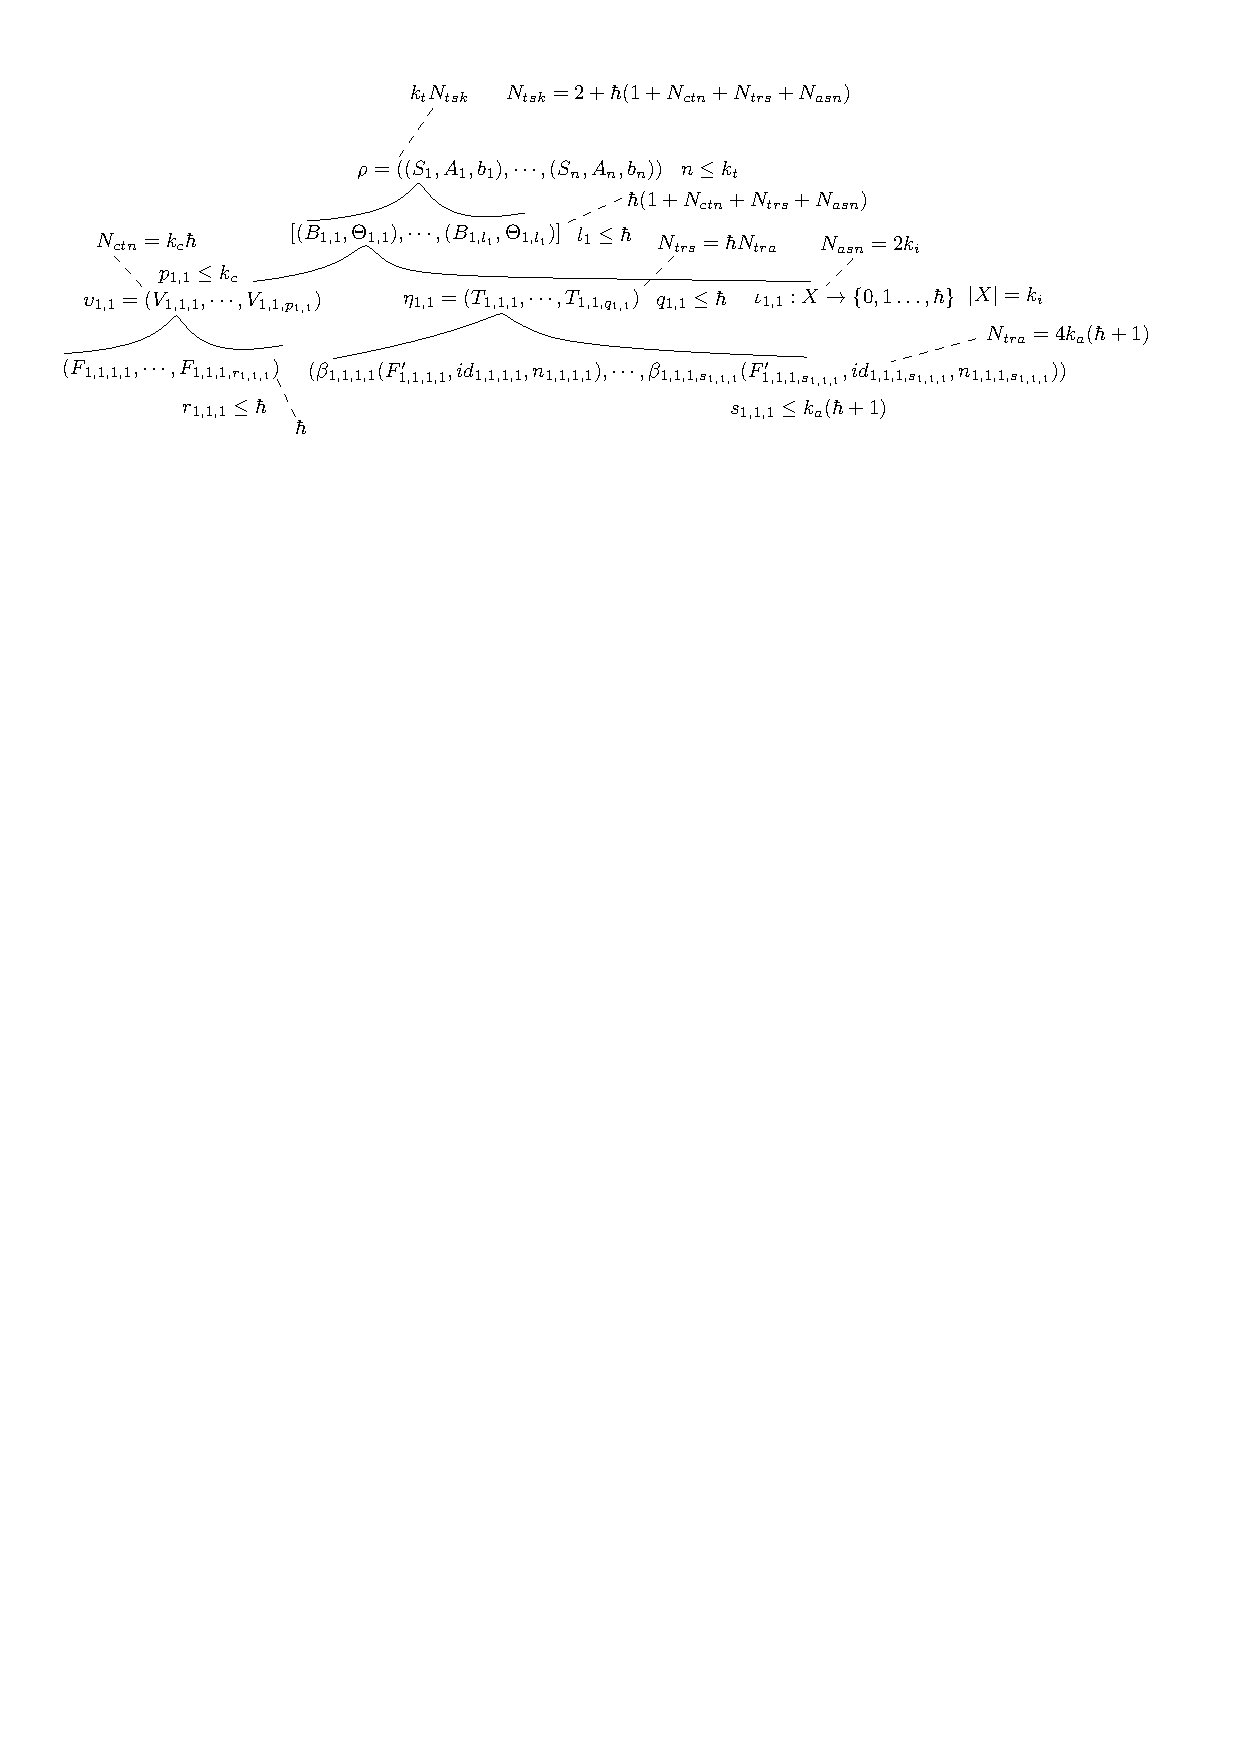
\includegraphics[scale = 0.7]{conf-enc-length.pdf}
\caption{Length of the word encoding a task stack}
\label{fig-conf-enc}
\end{figure*}

More specifically, we have that 
\begin{itemize}
\item each fragment container is encoded by a word of length $N_{ctn} =  k_c \hbar$, 
%
\item each transaction is encoded by a word of length $N_{tra} = 4k_a(\hbar+1)$, 
%
%\item $N_{tra} = 3k_a(\hbar+1)$ denote the length of the encoding of a transaction, 
\item each transaction stack is encoded by a word of length $N_{trs} = \hbar N_{tra}$, 
%
\item each assignment function is encoded by a word of length $N_{asn} = 2k_i $, i.e. a word of the form $x_1 n_1 \cdots x_{k_i} n_{k_i}$ (where $x_j \in X$ and $n_j \in \{0\} \cup [k_c\hbar]$), 
%
\item each activity is encoded by a word of length $N_{act} = 1+ N_{ctn} + N_{trs}+N_{asn}$, and
\item each task is encoded by a word of length $N_{tsk} =2+ \hbar N_{act}$.
\end{itemize}
Note that in the encoding, the top activity of the top task is in the first position.

We can then use $k_t N_{tsk}$ variables $X_1, \cdots, X_{k_t N_{tsk}}$ ranging over $\Sigma_\Mm$  to encode a task stack. 
Evidently, each symbol in $\Sigma_{\Mm}$ can be encoded as a bit vector of length $\log_2 |\Sigma_\Mm|$. For each $\sigma \in \Sigma_\Mm$, assume $\enc(\sigma)$ is the binary encoding of $\sigma$. 
Each configuration can be encoded by 
$
k_t N_{tsk} \log_2 |\Sigma_\Mm|
$
Boolean variables. 
%It follows that each configuration $(\rho, \ell)$ can be encoded by 
%$
%(k_t N_{tsk} +1) \log_2 |\Sigma_\Mm| 
%$
%Boolean variables. 
%
Therefore, $\Aa_\Mm$ uses $
k_t N_{tsk}  \log_2 |\Sigma_\Mm| 
$ state variables to encode the configurations in $\conf_{\Mm,c_t, \hbar}$. 
Moreover, $\Aa_\Mm$ contains the input variables to encode the transition rules of $\Mm$.
Equipped with these state variables and input variables, we then encode the semantics of the transition rules of $\Mm$ into the transitions of $\Aa_\Mm$. 
% 
%Then details of $\Aa_\Mm$ are omitted and can be found in Appendix~\ref{app-enc-amass-trans}. 


%%%%%%%%%%%%%%%%%%%%%%%%%%%%%%%%%%
%%%%%%%%%%%%%%%%%%%%%%%%%%%%%%%%%%

